\section{Prior Work}\label{sec:background_prior_work}

There have been several past attempts at evaluating \us internet connectivity, including an \mqp several years ago.

\subsection{FCC fixed broadband deployment map}
The \FCC maintains a map of broadband internet deployment across the United States \cite{FederalCommunicationsCommission}. This map is drawn at a census block level and only considers residential broadband.
 
 \subsection{Internet Connectivity MQP 2018}
In 2018, another \mqp was run at \wpi, also with the goal of mapping the internet connectivity across the United States. They used traceroutes from Worcester to top websites, and also performed \dns cache manipulation to collect their data. They had mixed success collecting data, but they were ultimately able to produce a map of all their \dns data interpolated to cover the entire \us, shown in \cref{fig:interpolated_dns_map}. They did not come to any conclusions as to the best or worst states \cite{Fakult2019}.

The core concept of \dns cache manipulation was ultimately used in our own research into evaluating and ranking internet connectivity, discussed in \cref{sec:dns}.

\begin{figure}[h]
    \centering
    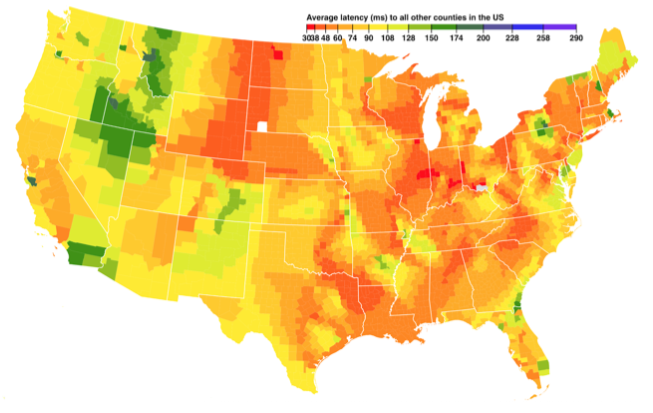
\includegraphics[width=\textwidth]{dns/prior_mqp/dns-map.png}
    \caption{Interpolated DNS map}
    \label{fig:interpolated_dns_map}
\end{figure}
 
\subsection{Physical Mapping of the Internets Fiber Backbone in the United States}
In 2015 researchers at the University of Wisconsin (Madison) set out to map the locations of the fiber backbone within the \us.  Their goal was to understand how the physical locations of the fiber backbone had been influenced by previous infrastructure such as railroads and the highway network. They found strong correlation between the location of fiber lines and the locations of major roads built in the mid 20th century. This result is significant for internet connectivity because it further highlights that cities that were well connected physically during the industrial revolution continue to be the best connected.
 